%%%%%%%%%%%%%%%%%%%%%%%%%%%%%%%%%%%%%%%%%
% Short Sectioned Assignment
% LaTeX Template
% Version 1.0 (5/5/12)
%
% This template has been downloaded from:
% http://www.LaTeXTemplates.com
%
% Original author:
% Frits Wenneker (http://www.howtotex.com)
%
% License:
% CC BY-NC-SA 3.0 (http://creativecommons.org/licenses/by-nc-sa/3.0/)
%
%%%%%%%%%%%%%%%%%%%%%%%%%%%%%%%%%%%%%%%%%

%----------------------------------------------------------------------------------------
%	PACKAGES AND OTHER DOCUMENT CONFIGURATIONS
%----------------------------------------------------------------------------------------

\documentclass[paper=a4, fontsize=11pt]{scrartcl} % A4 paper and 11pt font size

\usepackage[T1]{fontenc} % Use 8-bit encoding that has 256 glyphs
\usepackage{fourier} % Use the Adobe Utopia font for the document - comment this line to return to the LaTeX default
\usepackage[english]{babel} % English language/hyphenation
\usepackage{amsmath,amsfonts,amsthm} % Math packages
\usepackage{pgfplots, tikz,comment}
\usetikzlibrary{intersections}
\usepackage[CJKbookmarks=true,
            colorlinks,linkcolor=black,anchorcolor=blue,citecolor=green]{hyperref}

\usepackage{lipsum} % Used for inserting dummy 'Lorem ipsum' text into the template

\usepackage{sectsty} % Allows customizing section commands
\allsectionsfont{\centering \normalfont\scshape} % Make all sections centered, the default font and small caps

\usepackage{fancyhdr} % Custom headers and footers
\pagestyle{fancyplain} % Makes all pages in the document conform to the custom headers and footers
\fancyhead{} % No page header - if you want one, create it in the same way as the footers below
\fancyfoot[L]{} % Empty left footer
\fancyfoot[C]{} % Empty center footer
\fancyfoot[R]{\thepage} % Page numbering for right footer
\renewcommand{\headrulewidth}{0pt} % Remove header underlines
\renewcommand{\footrulewidth}{0pt} % Remove footer underlines
\renewcommand\thesection{\roman{section}}

\setlength{\headheight}{13.6pt} % Customize the height of the header

\numberwithin{equation}{section} % Number equations within sections (i.e. 1.1, 1.2, 2.1, 2.2 instead of 1, 2, 3, 4)
\numberwithin{figure}{section} % Number figures within sections (i.e. 1.1, 1.2, 2.1, 2.2 instead of 1, 2, 3, 4)
\numberwithin{table}{section} % Number tables within sections (i.e. 1.1, 1.2, 2.1, 2.2 instead of 1, 2, 3, 4)

\setlength\parindent{0pt} % Removes all indentation from paragraphs - comment this line for an assignment with lots of text

%----------------------------------------------------------------------------------------
%	TITLE SECTION
%----------------------------------------------------------------------------------------

\newcommand{\horrule}[1]{\rule{\linewidth}{#1}} % Create horizontal rule command with 1 argument of height

\title{	
\normalfont \normalsize
\textsc{School of Software, Tsinghua University} \\ [25pt] % Your university, school and/or department name(s)
\horrule{0.5pt} \\[0.4cm] % Thin top horizontal rule
\huge Optimization Method\\ % The assignment title
\LARGE\textit{homework 7}
\horrule{2pt} \\[0.5cm] % Thick bottom horizontal rule
}

\author{Qingfu Wen \\ \normalsize 2015213495} % Your Info
\date{\normalsize\today} % Today's date or a custom date

\begin{document}

\maketitle % Print the title
\tableofcontents
\newpage
%----------------------------------------------------------------------------------------
%	PROBLEM 1
%----------------------------------------------------------------------------------------
\section{Problem 1}
Solve the following 0-1 programming problem:
\begin{alignat}{2}          \nonumber
\min\quad & 2x_1+3x_2+4x_3 \\    \nonumber
\mbox{s.t.}\quad            \nonumber
& -3x_1+5x_2-2x_3 \geq -4\\
& 3x_1+x_2+4x_3 \geq 3\\
& x_1+x_2 \geq 1\\
& x_1,x_2,x_3\in \{0,1\}
\end{alignat}\\
\emph{\textbf{Solution:}}
\begin{itemize}
\item First, we can try a feasible solution $(1,1,0)$, $f_{min} = 5$.
\item we can list all possible solution by enumeration and validate it by constraint condition and present $f_{min}$.\\
\begin{tabular}{|c|c|c|c|c|c|}
\hline point&present $f_{min}$&1&2&3&f\\
\hline(0,0,0)&5&Y&N&&\\
\hline(1,0,0)&5&Y&Y&Y&2\\
\hline(0,1,0)&2&Y&N&&\\
\hline(0,0,1)&2&Y&Y&Y&4\\
\hline(1,1,0)&2&Y&Y&Y&5\\
\hline(1,0,1)&2&N&&&\\
\hline(0,1,1)&2&Y&Y&Y&7\\
\hline(1,1,1)&2&Y&Y&Y&9\\
\hline
\end{tabular}\\
\end{itemize}
Above all, we can see the optimal solution is $(1,0,0)$, $f_{min}=2$.

\section{Problem 2}
Suppose a factory produce two kind of products, product 1 and product 2, and each product's profits are respectively 15 and 25 (hundred yuan). Producing these products need production line A and production line B. For producing one product 1, it takes 1 hour on each line A and line B. For producing one product 2, it takes 3 hours on line A and 1 hour on line B. When making production plan, we need to consider:
\begin{enumerate}
\item $P_1$: profits of every week are no less than 750.
\item $P_2$: number of product 1 produced every week are no less than 25, product 2 are no less than 10.
\item $P_3$: work time of line A is no more than 60 hours and line B is no more than 40 hours, or the expense of line A is 3 times than line B for working another hour.
\end{enumerate}
Please model this problem by goal programming.\\\\
\emph{\textbf{Solution:}}\\
\begin{alignat}{2}          \nonumber
\min\quad & P_1d_1^-+P_2(d_2^-+d_3^-)+P_3(3d_4^++d_5^+) \\    \nonumber
\mbox{s.t.}\quad            \nonumber
& 15x_1+25x_2+d_1^--d_1^+ = 750\\        \nonumber
& x_1+d_2^--d_2^+ = 25\\                \nonumber
& x_2+d_3^--d_3^+ = 10\\              \nonumber
& x_1+3x_2+d_4^--d_4^+ = 60\\            \nonumber
& x_1+x_2+d_5^--d_5^+ = 40\\             \nonumber
& x_1,x_2,d_i^-,d_i^+ \geq 0, i=1,\cdots,5
\end{alignat}

\section{Problem 3}
Solve the following goal programming problem using graph method:
\begin{alignat}{2}          \nonumber
\min\quad & P_1d_1^-+P_2(d_2^-+d_3^-)+P_3(3d_4^++d_5^+) \\    \nonumber
\mbox{s.t.}\quad            \nonumber
& 15x_1+25x_2+d_1^--d_1^+ = 750\\        \nonumber
& x_1+d_2^--d_2^+ = 25\\                \nonumber
& x_2+d_3^--d_3^+ = 10\\              \nonumber
& x_1+3x_2+d_4^--d_4^+ = 60\\            \nonumber
& x_1+x_2+d_5^--d_5^+ = 40\\             \nonumber
& x_1,x_2,d_i^-,d_i^+ \geq 0, i=1,\cdots,5
\end{alignat}\\
\emph{\textbf{Solution:}}\\

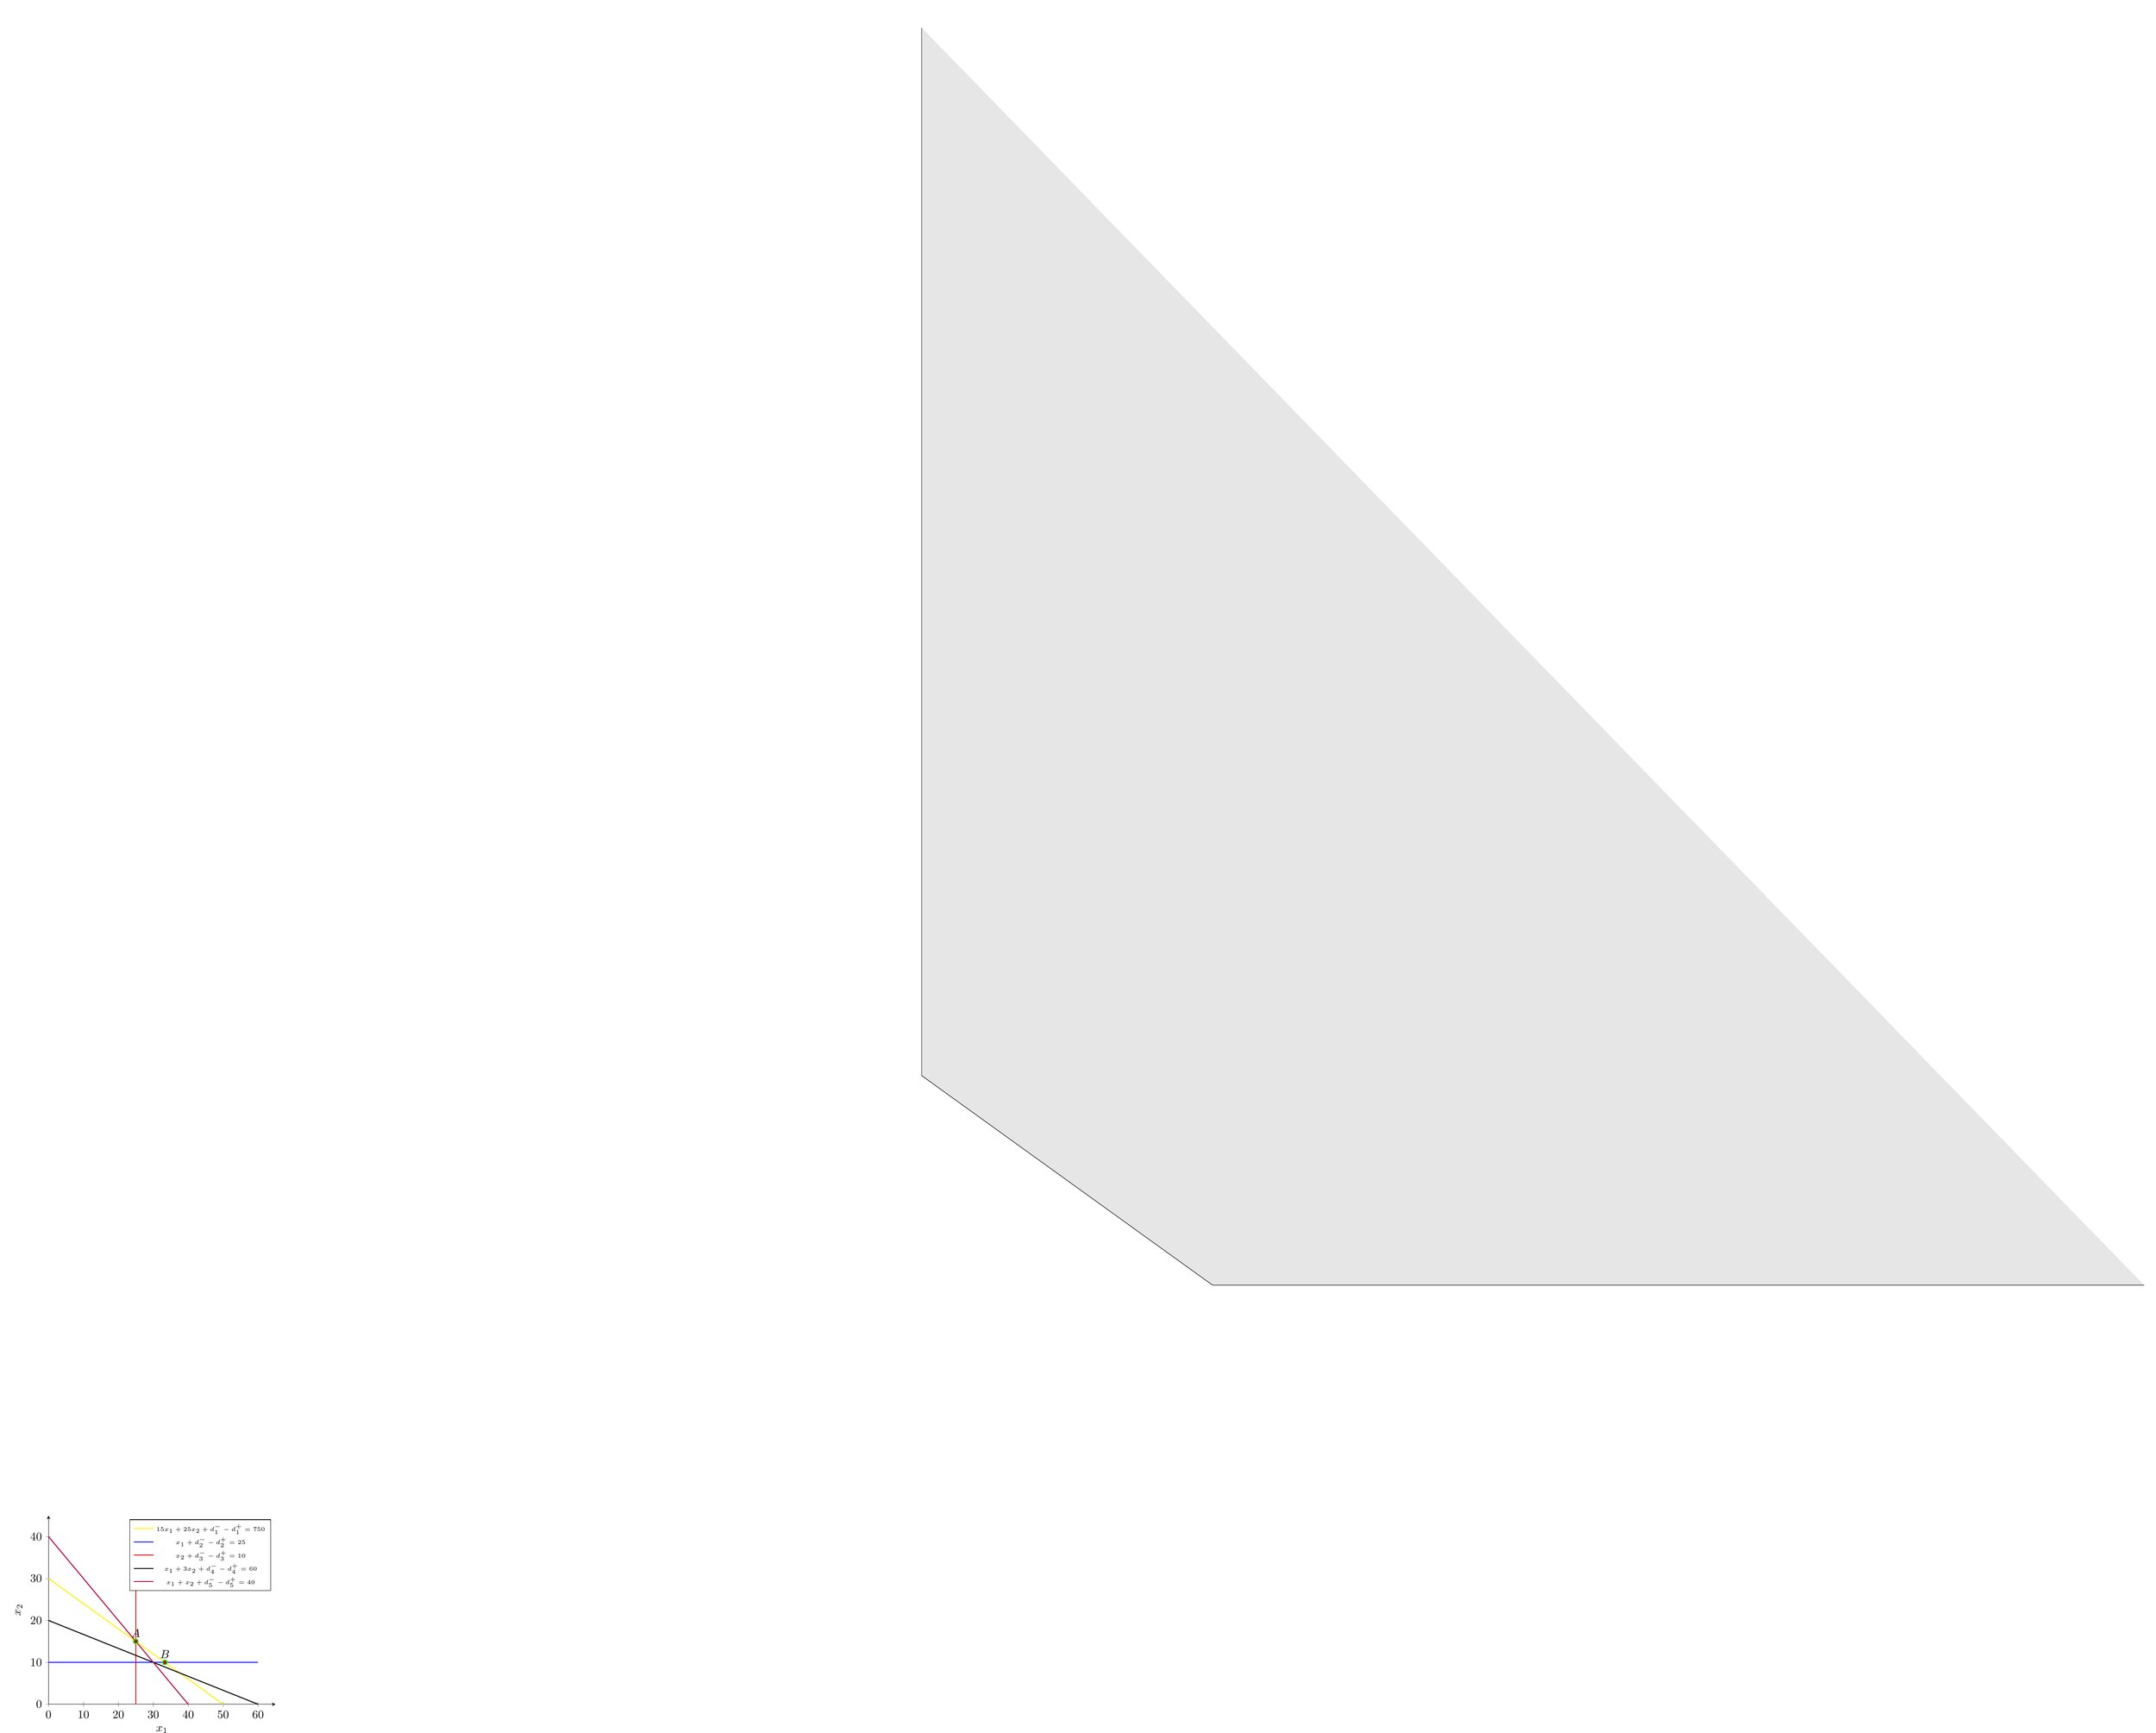
\begin{tikzpicture}
\begin{axis}[
    clip=false,
    xlabel=$x_1$,
    ylabel=$x_2$,
    axis x line=bottom,
    axis y line=left,
    no markers,
    ymin=0,
    xmin=0,
    xmax=65,
    ymax=45,
    legend style={font=\tiny},
    ]
    \addplot+[name path=one, domain=0:50,color=yellow,thick] {30-0.6*x};
    \addlegendentry{$15x_1+25x_2+d_1^--d_1^+ = 750$};
    \addplot+[name path=two, domain=0:60,color=blue,thick] {10};
    \addlegendentry{$x_1+d_2^--d_2^+ = 25$};
    \addplot+[name path=three,color=red,thick] coordinates {(25,0) (25,40)};
    \addlegendentry{$x_2+d_3^--d_3^+ = 10$};
    \addplot+[name path=four, domain=0:60,color=black,thick] {20-x/3};
    \addlegendentry{$x_1+3x_2+d_4^--d_4^+ = 60$};
    \addplot+[name path=five, domain=0:40,color=purple,thick] {40-x};
    \addlegendentry{$x_1+x_2+d_5^--d_5^+ = 40$};

    \draw [fill=gray,scale=10,fill opacity=0.2] (25,40) -- (25,15) -- (33.33,10) -- (60,10);

    \addplot+[name path=six,color=green,thick,only marks] coordinates {(25,15)(33.33,10)};
    \coordinate (O) at (axis cs:0,0);
    \draw[dashed,name intersections={of=one and three,name=i}] (i-1) node[above] {$A$};
    \draw[dashed,name intersections={of=one and two,name=i}] (i-1) node[above] {$B$};
  \end{axis}
\end{tikzpicture}\\
Considering constraint condition $P_1$ and $P_2$, the solution is in the gray area. By adding $P_3$, we can see the optimal solution is $B(33.33, 10)$.
\end{document}
